\documentclass[11pt,letterpaper]{article}
\usepackage[margin=0.78in,headheight=15pt]{geometry}
\usepackage[T1]{fontenc}
\usepackage{mathptmx,amsmath,amssymb,graphicx,booktabs,tabularx,longtable,array}
\usepackage[dvipsnames]{xcolor}
\usepackage{enumitem,caption,float,fancyhdr}
\usepackage[hyphens]{url}
\usepackage[colorlinks=true,linkcolor=MidnightBlue,urlcolor=MidnightBlue]{hyperref}
\hypersetup{pdftitle={T-RECAP Recorded RF Verification Supplement},pdfauthor={T-RECAP Senior Design Project}}
\definecolor{ink}{HTML}{17384C}
\definecolor{teal}{HTML}{147D81}
\definecolor{muted}{HTML}{52616D}
\pagestyle{fancy}
\fancyhf{}
\lhead{\small T-RECAP \quad Recorded RF verification}
\rhead{\small TRF1 profile}
\cfoot{\small\thepage}
\renewcommand{\headrulewidth}{0.3pt}
\setlength{\parindent}{1.2em}
\setlength{\parskip}{4pt}
\setlength{\emergencystretch}{2em}
\captionsetup{font=small,labelfont=bf}
\setlist[itemize]{leftmargin=1.3em,itemsep=3pt,topsep=3pt}
\setlist[enumerate]{leftmargin=1.6em,itemsep=4pt,topsep=3pt}
\newcolumntype{Y}{>{\raggedright\arraybackslash}X}
\newcommand{\atlas}[2]{\begin{figure}[H]\centering\includegraphics[width=\linewidth,height=3.4in,keepaspectratio]{../../architecture/rf_iq/#1.png}\caption{#2}\end{figure}}
\newcommand{\artifact}[1]{\nolinkurl{#1}}
\newcommand{\scopebox}[1]{\noindent\fcolorbox{ink!25}{ink!4}{\parbox{0.96\linewidth}{\small #1}}\par}

\begin{document}
\begin{center}
{\Large\bfseries\color{ink} Recorded RF I/Q Integration}\par\vspace{4pt}
{\large Design Verification and Implementation Supplement}\par\vspace{8pt}
{\normalsize T-RECAP Senior Design Project}\par\vspace{3pt}
{\small Threshold-based Reduction and Encoding for Controlled Audio Processing}\par\vspace{6pt}
{\small Verification refresh: 4 November 2026}
\end{center}

\begin{abstract}
This supplement evaluates a recorded radio-frequency input profile that converts complex unsigned eight-bit I/Q samples into the real signed twelve-bit stream accepted by the existing T-RECAP processor. Verification combines an independent integer convolution model, self-checking RTL simulation, application-register regressions, preserved implementation evidence and an earlier five-epoch physical FPGA capture. The new publication regression is identified separately from the historical hardware session. The demonstrated result is numerical and interface compatibility with the existing FFT, threshold, reconstruction and spectral-packet paths. It is not a claim of live RF reception, general protocol preservation, reduced CPU power or a new formal proof of the RF adapter.
\end{abstract}

\section{Objective and verification boundary}
The extension allows a recorded complex RF signal to use an established real-signal processing architecture. It adds input conversion, finite-record management and a distinct application interface named TRF1. The existing numerical core remains the processing baseline. The review asks whether the converter implements its specified arithmetic, whether accepted samples survive stalls and recovery correctly, and whether the application returns the same numerical outputs as an independently prepared real-sample input.

\begin{figure}[H]\centering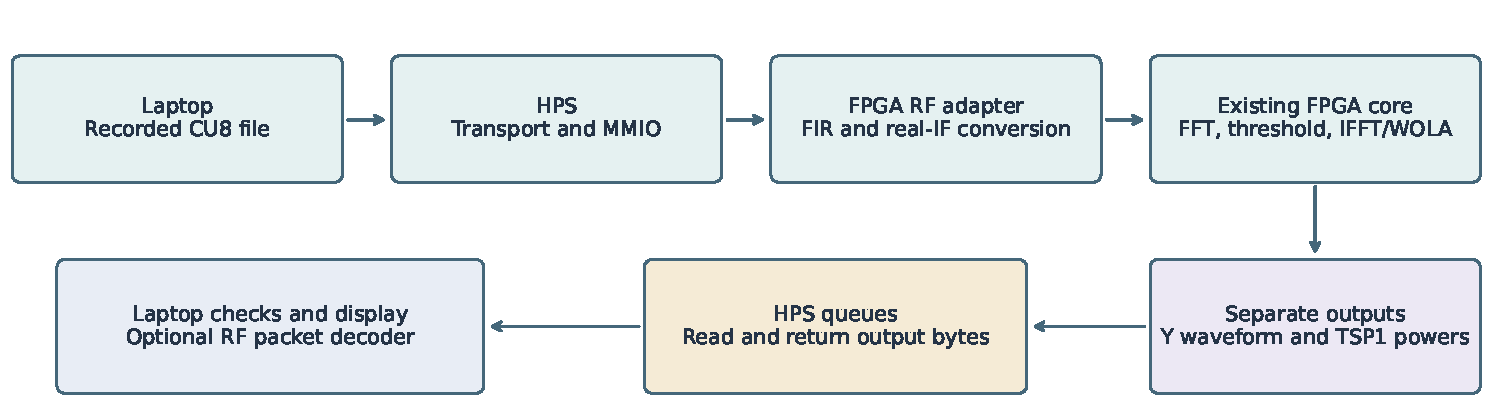
\includegraphics[width=\linewidth]{figures/system_boundary.pdf}
\caption{System boundary for recorded-file RF processing. The HPS transports bytes and commands. The detailed companion is \href{../../architecture/rf_iq/01-system.png}{atlas view 1}.}\end{figure}

\scopebox{Three evidence classes remain separate throughout this report. Fresh simulation validates the published source and tests. Historical implementation evidence identifies a particular fitted image. Historical physical captures record what that image produced during a specific earlier board session. None describes the image currently active on a board.}

\newpage
\section{Numerical contract}
Each input pair contains unsigned bytes $b_I,b_Q\in[0,255]$. Centering produces signed nine-bit values
\begin{equation}
d_I=2b_I-255,\qquad d_Q=2b_Q-255.
\end{equation}
The corresponding normalized values are $d_I/256$ and $d_Q/256$. Bytes 127 and 128 lie on opposite sides of zero. The finite-record flush therefore inserts exact zeros after centering rather than treating either byte as zero.

An 81-tap low-pass interpolation prototype is quantized to signed 18-bit coefficients with 16 fractional bits. The reference inserts three zeros between input samples and performs full integer convolution independently for I and Q. After compensating the 40-output-sample group delay, the quarter-rate mixer produces
\begin{equation}
u[n]=\operatorname{Re}\left\{\big(I_{4x}[n]+jQ_{4x}[n]\big)e^{j\pi n/2}\right\}.
\end{equation}
This selects $+I_{4x},-Q_{4x},-I_{4x},+Q_{4x}$ on successive phases. The four values occur at successive interpolated sample times. They are not four copies of one raw pair. The mixer preserves both I and Q in a real intermediate-frequency representation within the filter and quantization limits.

\begin{table}[H]\centering\small
\caption{Specified arithmetic and record geometry.}
\begin{tabularx}{\linewidth}{@{}p{1.9in}Y@{}}\toprule
Property & Contract \\ \midrule
Input record & $1\leq N\leq96{,}000$ unsigned I/Q pairs \\
Interpolating FIR & 81 coefficients, four phases, 21 scheduled positions per phase \\
Product and accumulator & Signed 27-bit product and signed 36-bit accumulation \\
Gain parameter & $g\in\{0,1,2,3\}$, divisor $2^{16-g}$ after accumulation \\
Final rounding & Nearest integer with exact half ties away from zero \\
Output quantization & Saturate to $[-2048,2047]$ and record each clipping event \\
Finite alignment & Discard 40 startup outputs and supply ten zero I/Q pairs internally \\
Valid output length & Exactly $4N$ accepted scalar samples \\
Application transaction & Append zeros to 384,000 real samples for the full board profile \\
\bottomrule\end{tabularx}
\end{table}

For the historical fixture, 250,000 complex samples per second become an equivalent one million real samples per second with an intermediate frequency of 250 kHz. These are signal-representation rates. They do not state the execution throughput of the sequential converter. The original 433.92 MHz carrier was already downconverted by the receiver that created the file.

\noindent The complete representation flow appears in \href{../../architecture/rf_iq/02-signal-representation.png}{atlas view 2}. Sample-rate conversion and real-IF translation operate on recorded baseband data. The finite interpolation filter, fixed-point coefficients and final quantization are part of the conversion error budget.

\newpage
\section{RTL architecture and transaction control}
The implementation schedules one shared multiplication and accumulation path. The FIR coefficient address is $4k+p$, where $k$ selects one of 21 history positions and $p$ selects the output phase. The coefficient function returns zero beyond the 81-tap prototype. Even phases read I history and odd phases read Q history. Applying the phase sign after accumulation removes the need for a separate general-purpose oscillator multiplier.

\begin{figure}[H]\centering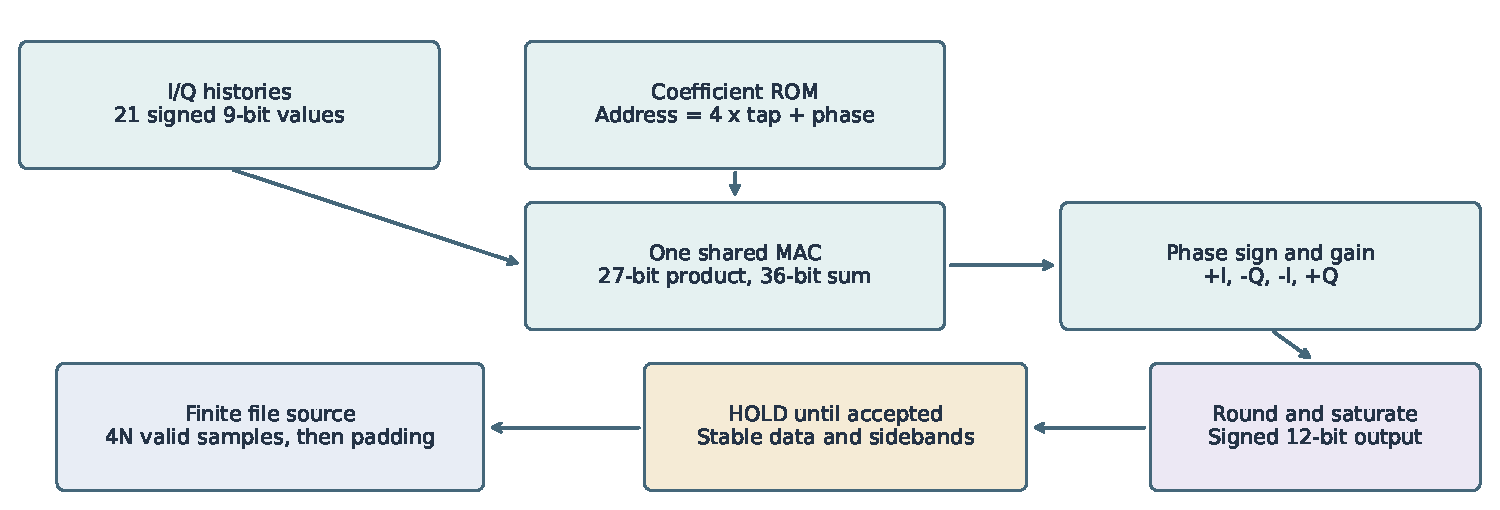
\includegraphics[width=\linewidth]{figures/adapter_schedule.pdf}
\caption{Scheduled RF datapath and output contract. The coefficient ROM and histories jointly feed the shared MAC. The detailed wiring and widths appear in \href{../../architecture/rf_iq/03-adapter-hardware.png}{atlas view 3}.}\end{figure}

\begin{table}[H]\centering\small
\caption{Adapter state-machine responsibilities.}
\begin{tabularx}{\linewidth}{@{}p{0.72in}Y@{}}\toprule
State & Observable responsibility \\ \midrule
IDLE & Admit a valid count and gain. Configuration is retained for the transaction. \\
LOAD & Accept a pair only on valid and ready. Shift I and Q histories or supply a zero flush pair. \\
MAC & Accumulate the 21 scheduled products for the current phase. \\
MAKE & Apply phase sign, gain, rounding and saturation. Discard the startup transient when required. \\
HOLD & Keep data and sideband outputs stable until the consumer accepts the sample. \\
\bottomrule\end{tabularx}
\end{table}

The source wrapper separates the valid $4N$ prefix from transaction padding. The application wrapper adds a 256-pair input FIFO, register validation, output queues and a transaction watchdog. Registered FIFO reads require an explicit pending stage and held pair. A pop request cannot be treated as immediately available data.

Reset and clear abort a transaction. The downstream finite-stream processor must also be cleared when a transaction is abandoned. Adapter completion and application completion are different events. Application DONE verifies input and production counts, but the host must still drain and validate any output retained in its FIFOs.

\newpage
\section{Verification methodology and requirement traceability}
The numerical oracle uses full convolution rather than the RTL's polyphase schedule. This reduces the chance of repeating a scheduling error in both implementation and checker. The scoreboard compares every accepted output sample and its clipping flag, index and last marker. It also checks counters after handshakes. A deliberately corrupted expected sample must fail the regression, providing a negative control for checker effectiveness.

At integration level, independently generated real PCM feeds the established application while raw I/Q feeds TRF1. Both paths instantiate the actual numerical core. Equality is checked at the core input, reconstructed Y output and TSP1 byte stream. This demonstrates input conversion and interface equivalence. Since both paths share the same established core, it is not a new independent proof of FFT or IFFT arithmetic.

\begin{table}[H]\centering\footnotesize
\caption{Requirement-to-check matrix. A condition count is not a structural coverage percentage.}
\renewcommand{\arraystretch}{1.17}
\begin{tabularx}{\linewidth}{@{}p{0.45in}p{1.45in}Y >{\raggedright\arraybackslash}p{1.2in}@{}}\toprule
ID & Requirement & Executed mechanism & Evidence layer \\ \midrule
R01 & Correct byte centering & Extrema, 127/128, complements and single-pair oracle & Model and adapter \\
R02 & FIR ordering and phase & I/Q impulses at boundaries, complex tones of both signs, random data & Adapter scoreboard \\
R03 & Defined rounding & Positive and negative exact half ties, signed saturation bounds & Model and maximum file \\
R04 & All admitted gains & Numerical vectors at gains 0, 1, 2 and 3 & Adapter and integration \\
R05 & Exact record length & $4N$ outputs, startup crop, zero flush, minimum and maximum record & Adapter and wrapper \\
R06 & Stable stalled output & Random ready gaps, long stalls, release-edge checks & Adapter waveform/checker \\
R07 & Configuration retained & Active count/gain pins change without altering admitted transaction & Adapter \\
R08 & Invalid input blocked & Zero/oversized counts, malformed upper word bits, invalid gain & Adapter and MMIO \\
R09 & Correct padding & Exact valid prefix followed by zeros and endpoint marker & Wrapper and integration \\
R10 & FIFO correctness & Full queues, registered reads, held pairs and output backpressure & MMIO integration \\
R11 & Controlled recovery & Clear, stalled-output reset, watchdog and restart & Adapter and admission \\
R12 & Exact downstream data & Core-input, Y and TSP1 comparisons with independent PCM path & Actual-core integration \\
R13 & Trustworthy completion & PASS marker, explicit checker completion and negative control & Regression runner \\
R14 & Artifact identity & SHA-256 source binding and original receipt verification & Evidence audit \\
\bottomrule\end{tabularx}
\end{table}

The standalone suite also includes adversarial sign patterns that approach the FIR coefficient absolute-sum bound. Gain 1 is analytically bounded against clipping for all admissible CU8 inputs. Higher gains intentionally exercise clipping. Such stress counts describe arithmetic coverage, not quality loss in a representative RF application.

\newpage
\section{Executed simulation results}
The fresh publication run passed all five RTL layers. Its adapter negative control also failed as intended when one expected value was deliberately corrupted. Native host tests ran separately under the undefined-behavior sanitizer. No board was accessed by this refresh.

\begin{table}[H]\centering\small
\caption{Fresh publication verification. See the machine-readable projection for exact receipt identities.}
\begin{tabularx}{\linewidth}{@{}p{1.65in}Y@{}}\toprule
Layer & Executed result \\ \midrule
Adapter & 3 seeds, 120 transactions, 33,240 exact samples \\
Maximum record & 384,000 exact samples and signed clipping/rounding checks \\
Finite wrapper & 4 completed, 2 aborted, 264 sample checks \\
Actual-core MMIO & 32 epochs, 5,634,999 checks, 18 fault/abort cases \\
Admission and recovery & 4,260 checks over 16,193 cycles \\
Native host tests & 28 register-mock checks, 11 file cases and 4 numeric cases \\
\bottomrule\end{tabularx}
\end{table}

The fresh integration cases extend the prior matrix with a one-pair minimum record, legal gains 0 and 2, and the maximum legal 56-bit threshold. The admission extension exercises pending FIFO-prefetch recovery. These are specific executed cases, not an exhaustive cross-product claim.
Independent regeneration checked 42 numerical fixtures, 405,304 samples and all 81 FIR coefficients. The package checker rejected all 5 deliberately corrupted source or fixture variants.


The publication regression uses redistributable synthetic numerical fixtures. Earlier standalone evidence also exercised three short recorded fixtures that are retained locally. Those recordings are not redistributed with this report. Different fixture inventories produce different totals and must not be presented as one uninterrupted regression.

\begin{table}[H]\centering\small
\caption{Preserved earlier regression results, separate from the fresh publication run.}
\begin{tabularx}{\linewidth}{@{}p{1.65in}Y@{}}\toprule
Layer & Recorded accepted result \\ \midrule
Independent numerical model & Eight unit tests, coefficient bounds and floating alignment checks \\
Standalone adapter & Three seeds, 129 completed transactions, 70,104 exact sample comparisons \\
Maximum file & 96,000 input pairs and 384,000 exact output comparisons \\
Rounding and clipping stress & 53 nonsaturating half ties and 16,298 clipping flags checked \\
Finite wrapper & Four completed transactions, two aborts, 264 sample checks \\
Early actual-core integration & Four paired epochs at thresholds 0 and $10^8$ \\
Board MMIO integration & 24 numerical epochs, 4,314,643 checks and 1,438,154 bus transactions \\
Admission extension & 2,269 checks over 13,800 simulated clock cycles \\
\bottomrule\end{tabularx}
\end{table}

The earlier MMIO run observed 411,181 cycles with a full raw-I/Q FIFO, 639,808 with a full spectral FIFO, 607,656 with a full Y FIFO and 2,439,780 stalled RF-to-core cycles. These confirm that the exercised transaction reached the intended stress conditions. They do not establish exhaustive state, branch or toggle coverage.

Diagnostic review preserves existing compiler warnings. The earlier registered core compile had 415 warnings and zero errors. Reviewed categories concern existing net declarations, input-port kind and deferred combinational checks. Omitted simulation ports were confirmed to be observation outputs. This evidence is qualified as reviewed, not warning-free.

\newpage
\section{Waveform evidence and protocol reasoning}
\begin{figure}[H]\centering
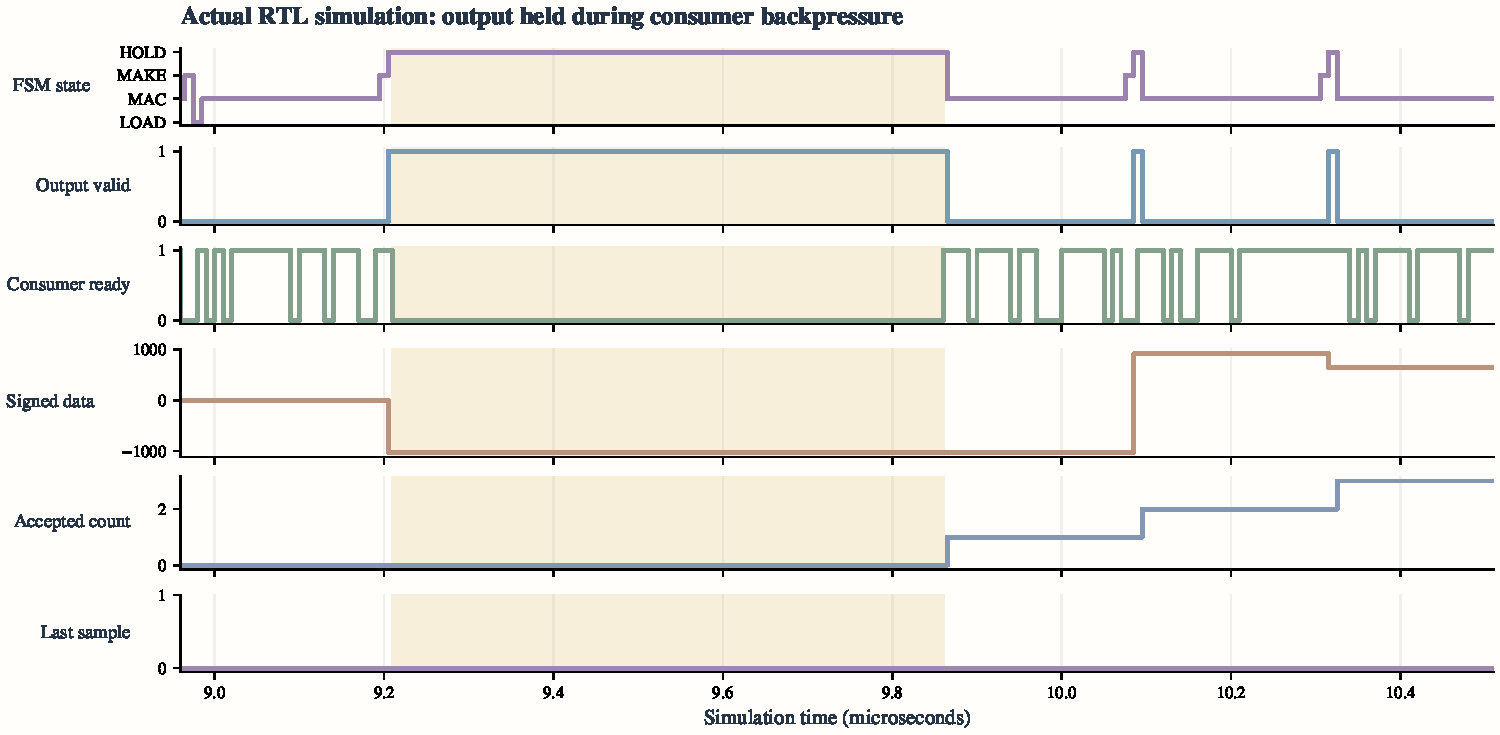
\includegraphics[width=\linewidth]{figures/rtl_backpressure.pdf}
\caption{A trace extracted from the fresh adapter RTL simulation. The shaded interval has valid asserted and consumer ready deasserted. The held data and accepted count remain stable. This is simulator evidence, not a physical logic-analyzer acquisition.}
\end{figure}

The trace includes the actual internal state and externally visible handshake values. During HOLD, the producer owns the presented sample. With ready low, advancing its sample index or replacing its data would lose information. Once ready permits acceptance, the count advances and the state machine may start the next scheduled phase. The checker applies the stability assertion through the release edge rather than checking only the middle of a stall.

The plotted interval is selected from the VCD and exported as a small CSV trace. The VCD digest, time unit, selected interval and trace digest are stored in \artifact{evidence/waveform_source.json}. The source waveform is the trace generated by the fresh regression, not an illustrative timing drawing.

\begin{table}[H]\centering\small
\caption{Boundary interpretation for the ready/valid contract.}
\begin{tabularx}{\linewidth}{@{}p{1.6in}Y@{}}\toprule
Condition & Expected behavior \\ \midrule
Input valid without ready & The upstream producer retains its pending pair. The adapter does not count an acceptance. \\
Output valid without ready & Data, clipping flag, index and last marker remain stable. \\
Clear during a stall & Transaction outputs are withdrawn and counters reset. The consumer is cleared as part of the enclosing abort. \\
Missing input & Standalone conversion waits. The application watchdog owns fault escalation and recovery. \\
DONE with queued results & The host continues draining validated output counts before considering retrieval complete. \\
\bottomrule\end{tabularx}
\end{table}

A short waveform illustrates one behavior. Confidence comes from the corresponding automated checks across the complete regression and from the directed recovery cases, not from visual inspection alone.

\newpage
\section{Implementation qualification}
The historical full TRF1 image targets Cyclone V 5CSEMA5F31C6 on DE1-SoC. It includes the HPS-connected application, RF conversion and existing numerical core. Its resource counts must not be confused with the earlier standalone adapter fit.

\begin{table}[H]\centering\small
\caption{Historical full-image resource use. Standalone adapter figures appear separately.}
\begin{tabular}{@{}lrr@{}}\toprule
Resource & Full TRF1 image & Device capacity \\ \midrule
Adaptive logic modules & 7,196 & 32,070 \\
Registers & 9,385 & \\
Block memory bits & 329,088 & 4,065,280 \\
M10K blocks & 48 & 397 \\
DSP blocks & 36 & 87 \\
Active pins & 138 & 457 \\
\bottomrule\end{tabular}
\end{table}

The isolated RF source assessment used 636 ALMs, 668 registers and one DSP block with no block RAM. It used virtual data/control pins and did not produce a board programming image. Its positive internal slack alone was not board timing signoff. The full implementation below has separate platform, pin, clock and DDR checks.

\begin{table}[H]\centering\small
\caption{Full-image 50 MHz fabric slack in nanoseconds.}
\begin{tabular}{@{}lrrrr@{}}\toprule
Corner & Setup & Hold & Recovery & Removal \\ \midrule
Slow 1.1 V, 85 $^\circ$C & 2.832 & 0.220 & 11.148 & 0.831 \\
Slow 1.1 V, 0 $^\circ$C & 2.685 & 0.211 & 11.370 & 0.760 \\
Fast minimum 1.1 V, 85 $^\circ$C & 10.387 & 0.130 & 14.588 & 0.481 \\
Fast minimum 1.1 V, 0 $^\circ$C & 11.053 & 0.112 & 14.953 & 0.430 \\
\bottomrule\end{tabular}
\end{table}

The implementation audit checked 18 expected clocks, 288 clock/check records and 32 calibrated DDR categories. All 127 HPS pins and 11 FPGA pins matched the qualified platform. Fifteen generated HPS handoff files matched the parent configuration byte for byte.

The fitter retained 338 warnings in the same eight reviewed categories as the qualified finite-stream build. Two critical messages concern hard HPS pin locations. Exact pin comparison and DDR checks independently passed. Hard-HPS model exceptions are explicitly classified and do not exempt fabric timing registers. The report therefore records reviewed implementation qualification without asserting that all diagnostic warnings were eliminated.

\scopebox{The fit and assembly are historical evidence tied to the image hash in Section~\ref{sec:evidence}. Fresh simulation does not create a new fitted image. No live RF rate, CPU speedup or electrical-power saving follows from the clock constraint or resource table.}

\newpage
\section{Historical physical qualification}
The earlier board session transferred an unchanged 131,072-byte CU8 file containing 65,536 complex samples. The FPGA admitted TRF1 with gain 1, converted 262,144 valid real samples and padded its input transaction to 384,000 samples. Each epoch produced 384,512 Y samples and 3,001 TSP1 frames. The HPS transported raw input and returned results. Golden PCM, Y and TSP1 files remained on the laptop.

Across five consecutive physical epochs, all 1,922,560 returned Y samples and 8,518,600 TSP1 bytes matched the independent adapter and qualified core references. Each run had zero adapter clips and zero dropped frames. Equal-threshold dense and sparse modes decoded to identical spectral values and returned identical Y waveforms.

\begin{table}[H]\centering\small
\caption{Earlier physical results over the valid-input interval. Packet savings use dense spectral packets as their baseline.}
\begin{tabular}{@{}rlrrr@{}}\toprule
Epoch & Threshold and mode & Spectral bytes & Savings (\%) & Relative L2 (\%) \\ \midrule
1 & 0 sparse & 2,212,920 & $-13.45$ & 0.000 \\
2 & $10^8$ dense & 1,950,648 & 0.00 & 0.353 \\
3 & $10^8$ sparse & 1,286,304 & 34.06 & 0.353 \\
4 & $10^{10}$ sparse & 792,192 & 59.39 & 8.086 \\
5 & $10^{11}$ sparse & 182,136 & 90.66 & 35.115 \\
\bottomrule\end{tabular}
\end{table}

\begin{figure}[H]\centering
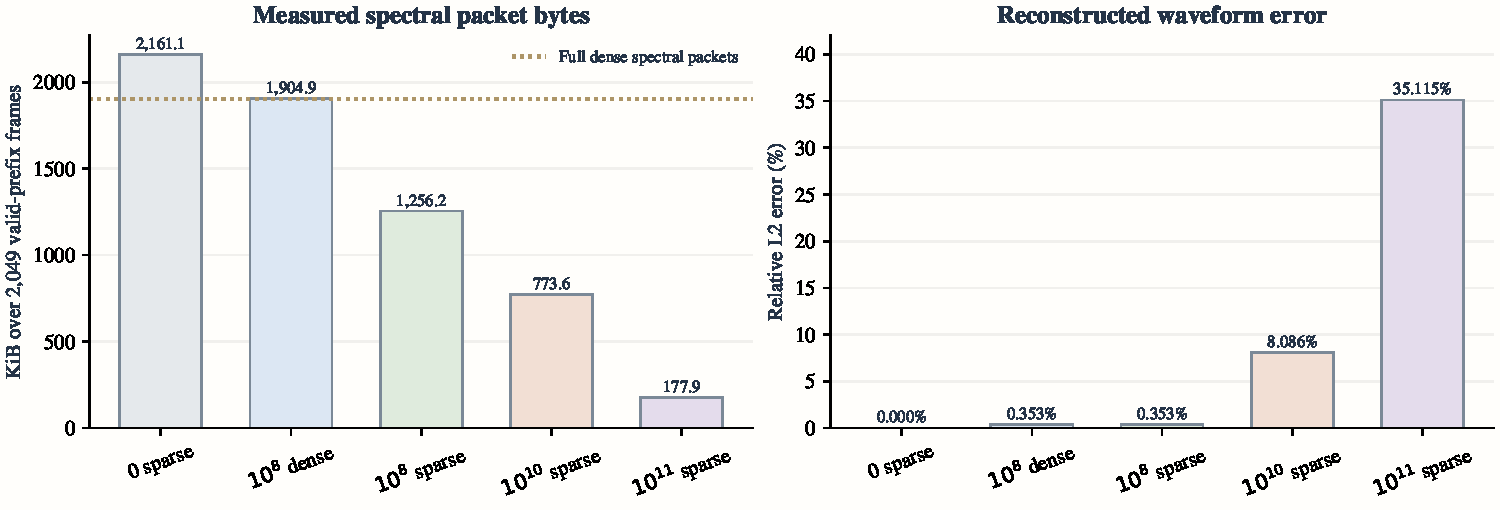
\includegraphics[width=\linewidth]{figures/historical_tradeoff.pdf}
\caption{Historical RF tradeoff from verified scalar results. The 2,049 frames touching valid input are counted. The additional 952 padding-only frames are excluded from headline savings.}
\end{figure}

The CPU decoder recovered the expected Rosenborg-66796 payload at every tested threshold. It uses I/Q recovered from Y. TSP1 contains power and bin metadata without phase, so it cannot independently reconstruct the waveform. This host-side decoder check covers one recorded civilian OOK transmission. Successful decoding of one payload does not guarantee preservation of weak signals or other protocols.

Sparse encoding has index overhead. At threshold zero it is larger than dense encoding. Even the smallest spectral packet result above exceeds the original 128 KiB raw file. The relative L2 error uses the fixed-point adapter reference as its baseline and excludes the adapter's own conversion error. Exact agreement with a thresholded numerical reference does not mean lossless reconstruction of the original signal.

\newpage
\section{Evidence identity and publication audit}\label{sec:evidence}
The historical evidence is bound through source registration, programming-image identity, programming receipt, capture receipt and returned-file hashes. A fresh local read-only audit verified 224 referenced artifact hashes before exporting the sanitized projection. That audit checks consistency of retained artifacts. It is not an independent digital signature or a second hardware acquisition.

\begin{table}[H]\centering\small
\caption{Exact historical artifact identities.}
\begin{tabularx}{\linewidth}{@{}p{1.15in}Y@{}}\toprule
Identity & Value \\ \midrule
SOURCE\_ID & \path{1f567ac68e2f8d3affd51e73c7dad1c144795df2045eeb290d33a806f8a9d700} \\
SOF SHA-256 & \path{3dd3cf18449ad6ad134b6782001406f67051e0401430fc96e19e07bf79728429} \\
Build registration & \path{8a422a028c262a1884e13642e0be42f4ca680e6850e8422217f4639542ad327d} \\
Capture receipt & \path{5e30afd799372ae98a6fd47d8661abb86667abda38fd0c54ef53445306b5cf62} \\
Program receipt & \path{20dc2e10e16a972ee6384ae2323c486b52ff72a0248680a2d358a7291dc105bd} \\
Linux boot UUID & \path{4836f67f-2b35-44f5-9b72-84bdbef17f45} \\
\bottomrule\end{tabularx}
\end{table}

The historical projection preserves each original receipt's digest and the five returned waveform and packet digests. It excludes absolute machine paths, raw recordings and large capture archives. It is explicitly labeled a projection rather than a verbatim original receipt. Published source files, figures and evidence are checked by the bundle manifest. The full local retained artifacts are required to repeat the historical-artifact audit.

The public sample identity is pinned to a specific \texttt{rtl\_433\_tests} repository commit. The original raw file is not redistributed because no redistribution permission is inferred. Fresh RTL verification uses generated numerical fixtures, allowing the test suite to run without that recording.

\subsection{Limits on verification claims}
\begin{itemize}
\item The new RF adapter and TRF1 interface have self-checking simulation evidence. No new RF formal proof or RF UVM environment is claimed.
\item Existing TSH2 formal and UVM work covers its documented earlier scope. Reusing core RTL does not automatically extend those results to the RF front end, FIFOs or register wrapper.
\item The application simulations use reduced transaction geometry. The maximum-length adapter test and historical physical full-geometry capture provide complementary evidence, not an exhaustive full-system proof.
\item Generated HPS bridges, ARM execution, DDR and Ethernet are outside the RTL integration simulation. Their historical platform and capture checks remain separately identified.
\item No structural code-coverage percentage, arbitrary RF protocol guarantee, live acquisition qualification, power result or downstream workload result is established here.
\end{itemize}

\newpage
\section{Reproduction and reviewer navigation}
The publication places RF RTL and the independent arithmetic model under \artifact{phase2/profiles/trf1}. The self-checking suite is under \artifact{phase2/verification/rf_iq}. Its runner records tool identity, source/fixture digests, commands, completion checks and evidence. The report directory contains LaTeX source, the compiled PDF, derived figures, sanitized historical evidence and a bundle checker.

\begin{enumerate}
\item Follow the suite README to select installed simulators and run the numerical model, adapter, maximum-length, wrapper, actual-core integration and admission checks into a fresh result directory.
\item Inspect the fresh summary and each layer's PASS marker. A simulator exit alone is insufficient. The deliberate corrupted-golden run must be reported as an expected failure.
\item Run \texttt{python check\_bundle.py} from this report directory to verify its manifest and linked figure/evidence files.
\item Build this document with two \texttt{pdflatex} passes using the supplied README. LaTeX compilation does not rerun the design tests.
\item Reproduce the historical projection only when the original local workspace artifacts are available. The export script accepts that workspace explicitly and does not access hardware.
\end{enumerate}

\begin{table}[H]\centering\small
\caption{Eight complementary architecture views shared with the updated atlas.}
\begin{tabularx}{\linewidth}{@{}p{0.35in}p{2.25in}Y@{}}\toprule
View & Figure & Question answered \\ \midrule
1 & \href{../../architecture/rf_iq/01-system.png}{System boundary} & Which work is on laptop, HPS and FPGA? \\
2 & \href{../../architecture/rf_iq/02-signal-representation.png}{Signal representation} & How do complex samples become a real IF stream? \\
3 & \href{../../architecture/rf_iq/03-adapter-hardware.png}{Adapter hardware} & How do history, coefficients and one MAC implement the converter? \\
4 & \href{../../architecture/rf_iq/04-finite-file-completion.png}{Finite-file completion} & How are valid data, tail and padding distinguished? \\
5 & \href{../../architecture/rf_iq/05-waveform-and-spectral-outputs.png}{Separate outputs} & What can Y and TSP1 each represent? \\
6 & \href{../../architecture/rf_iq/06-host-and-registers.png}{Host and registers} & How are commands, queues and application identity handled? \\
7 & \href{../../architecture/rf_iq/07-state-and-backpressure.png}{State and backpressure} & What changes on a handshake or during a stall? \\
8 & \href{../../architecture/rf_iq/08-clock-reset-verification.png}{Clock, reset and verification} & Which implementation boundaries and evidence layers apply? \\
\bottomrule\end{tabularx}
\end{table}

The appropriate senior-design conclusion is a verified recorded-file RF integration with explicit numerical, interface and implementation evidence. The architecture accepts a second representation of sampled signals while preserving its established processing core. Broader claims require a separately defined application metric, representative datasets and the corresponding hardware or software measurements.

\vfill
\noindent\small\textbf{Evidence navigation.}
\href{evidence/historical_projection.json}{Historical projection},
\href{evidence/waveform_source.json}{waveform provenance},
\href{../../../verification/rf_iq/README.md}{fresh regression guide},
\href{../../architecture/rf_iq/index.html}{interactive architecture atlas},
\href{README.md}{report build and audit instructions}.
\end{document}
